\documentclass[11pt,a4paper]{article}
\usepackage[utf8]{inputenc}
\usepackage{amsmath,enumitem,amsfonts,amssymb,graphicx,commath}
\usepackage{sectsty}
\usepackage{multicol}
\usepackage{tikz}
\usepackage{graphicx}

\usetikzlibrary{shapes,arrows,automata,arrows.meta}

\graphicspath{ {./img/} }
\DeclareMathAlphabet{\pazocal}{OMS}{zplm}{m}{n}

\usepackage[%
    left=1in,%
    right=1.0in,%
    top=1in,%
    bottom=1in,%
]{geometry}%

\sectionfont
{\fontsize{14.4}{12}\selectfont}
\title{\textbf{Principles of AI Planning
		\\{\Large Exercise Sheet 13}}}
\makeatletter
\renewcommand{\@maketitle}
{
	\newpage
	\null
	\vskip 2em%
	\begin{center}%
		{\LARGE \@title \\ \par}%
	\end{center}%
	\par
} \makeatother

\begin{document}
\begin{flushleft}
	Authors:\\
	Erick Rosete Beas | er165@uni-freiburg.de\\
	Jessica Lizeth Borja Diaz | jb986@uni-freiburg.de\\
\end{flushleft}
{\let\newpage\relax\maketitle}
\begin{center} 
	\large 07.02.2020
\end{center}


%%%%%%%%%%%%%%%%%%%%%  Ejercicio 1 %%%%%%%%%%%%%%%%%%%%%%%%%
\section*{Exercise 13.1 - EVMDDs}
(a)
\begin{multicols}{2}
	\begin{center}
		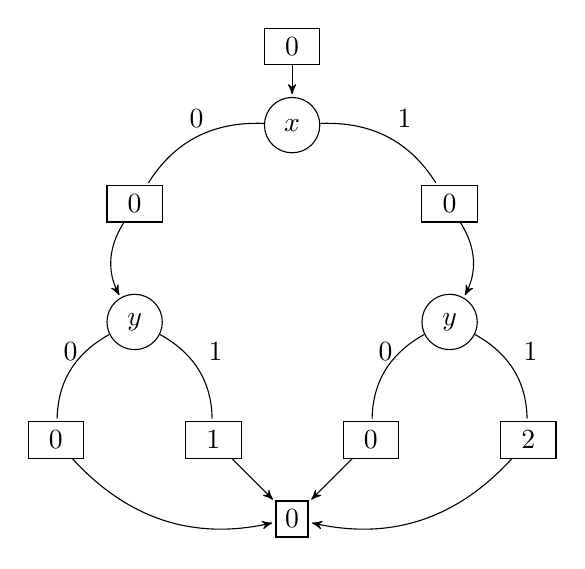
\begin{tikzpicture}
			\begin{scope}
				[
					styleVar/.style={
						minimum width = 2em, draw, circle,
						label={[above]#1}
						},
					styleCost/.style={minimum width = 2em, draw},
					end/.style={ minimum width = 0.2em, draw, thick},
				]
				\node(start)[styleCost] at (0,1) {$0$};
				\node(x)[styleVar] at (0,0) {$x$};
				\node(cx0)[styleCost] at (-2,-1) {$0$};
				\node(cx1)[styleCost] at (2,-1) {$0$};

				\node(y)[styleVar] at (-2,-2.5) {$y$};
				\node(cy0)[styleCost] at (-3,-4) {$0$};
				\node(cy1)[styleCost] at (-1,-4) {$1$};
				
				\node(yp)[styleVar] at (2,-2.5) {$y$};
				\node(cyp0)[styleCost] at (1,-4) {$0$};
				\node(cyp1)[styleCost] at (3,-4) {$2$};

				\node(end)[end] at (0,-5){$0$};
			\end{scope}
			\begin{scope}
				[ cost/.style = {->=stealth'},
				>=stealth',shorten >=1pt,auto]
				\path 
				(start) edge[cost]       		node{}(x)
				(x) edge[bend right, above]     node{$0$}(cx0)
				(x) edge[bend left]         	node{$1$}(cx1)
				(cx0) edge[bend right,cost]     node{}(y)
				(cx1) edge[bend left,cost]		node{}(yp)

				(y) edge[bend right, above]     node{$0$}(cy0)
				(y) edge[bend left]         	node{$1$}(cy1)
				(cy0) edge[bend right, cost]    node{}(end)
				(cy1) edge[cost]				node{}(end)

				(yp) edge[bend right, above]    node{$0$}(cyp0)
				(yp) edge[bend left]         	node{$1$}(cyp1)
				(cyp0) edge[cost]      		    node{}(end)
				(cyp1) edge[bend left, cost]    node{}(end);

			\end{scope}
		\end{tikzpicture}
	\end{center}
	\begin{center}
		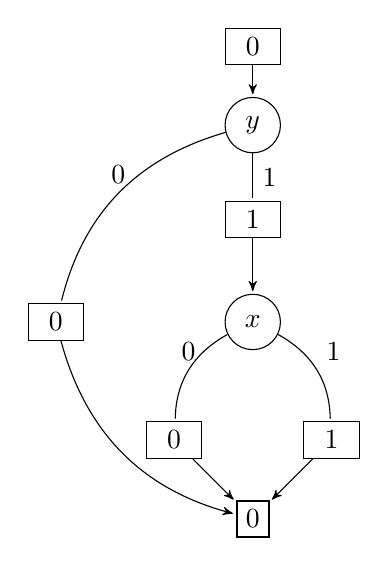
\begin{tikzpicture}
			\begin{scope}
				[
					styleVar/.style={
						minimum width = 2em, draw, circle,
						label={[above]#1},
						->=stealth'
						},
					styleCost/.style={minimum width = 2em, draw},
					end/.style={ minimum width = 0.2em, draw, thick},
				]
				\node(start)[styleCost] at (0,1) {$0$};
				\node(y)[styleVar] at (0,0) {$y$};
				\node(cy0)[styleCost] at (-2.5,-2.5) {$0$};
				\node(cy1)[styleCost] at (0,-1.2) {$1$};
	
				\node(x)[styleVar] at (0,-2.5) {$x$};
				\node(cx0)[styleCost] at (-1,-4) {$0$};
				\node(cx1)[styleCost] at (1,-4) {$1$};
				\node(end)[end] at (0,-5){$0$};
			\end{scope}
			
			\begin{scope}
				[ cost/.style = {->=stealth'},
					>=stealth',shorten >=1pt,auto]
				\path 
				(start) edge[cost] 					node{}(y)
				(y) edge[above, bend right]        	node{$0$}(cy0)
				(y) edge         					node{$1$}(cy1)
				(cy0) edge[bend right, cost]     	node{}(end)
				(cy1) edge[cost]			     	node{}(x)
	
				(x) edge[above,bend right]        	node{$0$}(cx0)
				(x) edge[bend left]         		node{$1$}(cx1)
				(cx0) edge[cost]				    node{}(end)
				(cx1) edge[cost]				    node{}(end);
	
			\end{scope}
		\end{tikzpicture}
	\end{center}
\end{multicols}
(b)
\begin{center}
	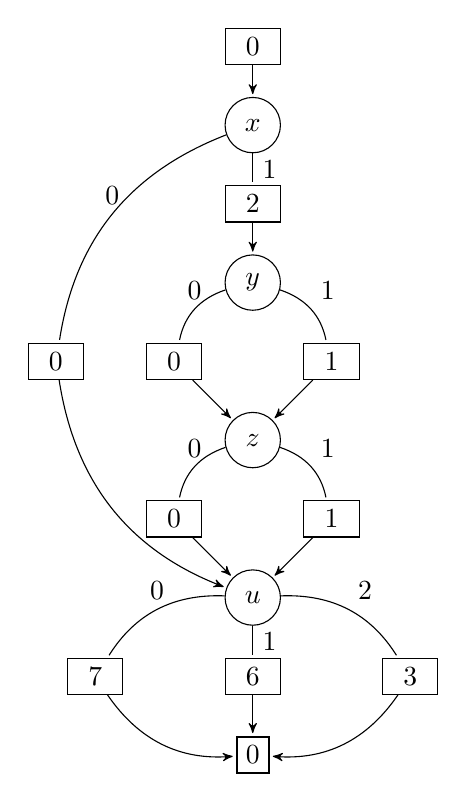
\begin{tikzpicture}
		\begin{scope}
			[
				styleVar/.style={
					minimum width = 2em, draw, circle,
					label={[above]#1},
					->=stealth'
					},
				styleCost/.style={minimum width = 2em, draw},
				end/.style={ minimum width = 0.2em, draw, thick},
			]
			\node(start)[styleCost] at (0,1) {$0$};
			\node(x)[styleVar] at (0,0) {$x$};
			\node(cx0)[styleCost] at (-2.5,-3) {$0$};
			\node(cx1)[styleCost] at (0,-1) {$2$};

			\node(y)[styleVar] at (0,-2) {$y$};
			\node(cy0)[styleCost] at (-1,-3) {$0$};
			\node(cy1)[styleCost] at (1,-3) {$1$};

			\node(z)[styleVar] at (0,-4) {$z$};
			\node(cz0)[styleCost] at (-1,-5) {$0$};
			\node(cz1)[styleCost] at (1,-5) {$1$};

			\node(u)[styleVar] at (0,-6) {$u$};
			\node(cu0)[styleCost] at (-2,-7) {$7$};
			\node(cu1)[styleCost] at (0,-7) {$6$};
			\node(cu2)[styleCost] at (2,-7) {$3$};

			\node(end)[end] at (0,-8){$0$};
		\end{scope}
		
		\begin{scope}
			[ cost/.style = {->=stealth'},
				>=stealth',shorten >=1pt,auto]
			\path 
			(start) edge[cost] 					node{}(x)
			(x) edge[bend right, above]        	node{$0$}(cx0)
			(x) edge         					node{$1$}(cx1)
			(cx0) edge[bend right, cost]     	node{}(u)
			(cx1) edge[cost]			     	node{}(y)

			(y) edge[bend right, above]        	node{$0$}(cy0)
			(y) edge[bend left]         		node{$1$}(cy1)
			(cy0) edge[cost]				    node{}(z)
			(cy1) edge[cost]				    node{}(z)

			(z) edge[bend right,above]        	node{$0$}(cz0)
			(z) edge[bend left]         		node{$1$}(cz1)
			(cz0) edge[cost]				    node{}(u)
			(cz1) edge[cost]				    node{}(u)

			(u) edge[bend right,above]        	node{$0$}(cu0)
			(u) edge			         		node{$1$}(cu1)
			(u) edge[bend left]         		node{$2$}(cu2)
			(cu0) edge[bend right, cost]		node{}(end)
			(cu1) edge[cost]				    node{}(end)
			(cu2) edge[bend left,cost]			node{}(end);

		\end{scope}
	\end{tikzpicture}
\end{center}
%%%%%%%%%%%%%%%%%%%%%  Ejercicio 2 %%%%%%%%%%%%%%%%%%%%%%%%%
\section*{Exercise 13.2 - EVMDD sizes and variable orders}

Let $v_0,...,v_{2n-1}$ be variables with domains $\pazocal{D}_{v_i} = \{0,...,k-1\} \forall i = 0,...,2n-1$,
let $\pi:=\{0,...,2n-1\} \rightarrow \{0,...,2n-1\}$ be a permutation of the variables,
let $k_j \in \mathbb{N}, j=0,...,n-1,$ be natural numbers and let
$c = \Sigma_{j=0}^{n-1}k_jv_{\pi(2j)}v_{\pi(2j+1)}$ be an arithmetic
function over $v_0,...,v_{2n-1}$.Intuitively, $c$ is a weighted sum 
of products of two variables each, such that no variable occurs in
more than one product subterm. Show that there exists a variable order 
for $v_0,...,v_{2n-1}$ such
that there exists an EVMDD with that order that represents the 
function $c$ and that has a size (number of edges) in the order 
of $nk^2$.\\

\emph{Hint:} Consider the example $c=2v_0v_3 + 6v_1v_5 + 4v_2v_4$. How
should the variables be ordered to minimize the size of the EVMDD.
\begin{center}
	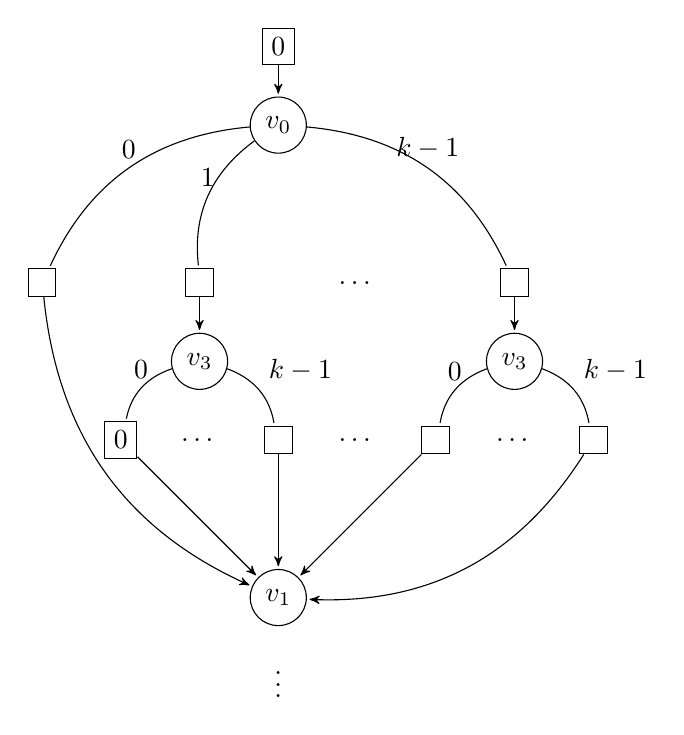
\begin{tikzpicture}
		\begin{scope}
			[
				styleVar/.style={
					minimum width = 2em, draw, circle,
					label={[above]#1},
					->=stealth'
					},
				styleCost/.style={minimum width = 1em, minimum height=1em, draw},
				end/.style={ minimum width = 0.2em, draw, thick},
			]
			\node(start)[styleCost] at (0,1) {$0$};
			\node(y)[styleVar] at (0,0) {$v_0$};
			\node(cy0)[styleCost] at (-3,-2) {};
			\node(cy1)[styleCost] at (-1,-2) {};
			\node(dots1) at (1,-2) {$\dots$};
			\node(cyk1)[styleCost] at (3,-2) {};

			\node(x)[styleVar] at (-1,-3) {$v_3$};
			\node(cx0)[styleCost] at (-2,-4) {$0$};
			\node(dots2) at (-1,-4) {$\dots$};
			\node(cx1)[styleCost] at (0,-4) {};

			\node(dots3) at (1,-4) {$\dots$};

			\node(z)[styleVar] at (3,-3) {$v_3$};
			\node(cz0)[styleCost] at (2,-4) {};
			\node(dots3) at (3,-4) {$\dots$};
			\node(cz1)[styleCost] at (4,-4) {};

			\node(v1)[styleVar] at (0,-6){$v_1$};

			\node(moreDots) at (0,-7) {$\vdots$};

		\end{scope}
		
		\begin{scope}
			[ cost/.style = {->=stealth'},
				>=stealth',shorten >=1pt,auto]
			\path 
			(start) edge[cost] 					node{}(y)
			(y) edge[above, bend right]        	node{$0$}(cy0)
			(y) edge[above, bend right]        	node{$1$}(cy1)
			(y) edge[above, bend left]        	node{$k-1$}(cyk1)
			(cy0) edge[bend right, cost]     	node{}(v1)
			(cy1) edge[cost]			     	node{}(x)
			(cyk1) edge[cost]			     	node{}(z)

			(x) edge[above,bend right]        	node{$0$}(cx0)
			(x) edge[bend left]         		node{$k-1$}(cx1)
			(cx0) edge[cost]				    node{}(v1)
			(cx1) edge[cost]				    node{}(v1)

			(z) edge[above,bend right]        	node{$0$}(cz0)
			(z) edge[bend left]         		node{$k-1$}(cz1)
			(cz0) edge[cost]					node{}(v1)
			(cz1) edge[bend left, cost]			node{}(v1);

		\end{scope}
	\end{tikzpicture}
\end{center}

for $c=2v_0v_3 + 6v_1v_5 + 4v_2v_4$ we consider the diagram above
which is a EVMDD for $c$. $v_0$ can take values from $0$ to $k-1$ 
hence that node has $k$ outcoming edges. And for $k-1$ edges that
branch out from $v_0$ there is a node $v_3$ with $k$ more edges.
Then for each pair $v_{\pi(2j)}v_{\pi(2j+1)}$ there exists $(k-1)k + 1$ edges
which is in order $O(k^2)$, and we have $n$ variable pairs 
which means the EVMDD has in total $O(n*k^2)$ edges.\\

Given arbitrary $n$ and $k$, using as variable order
the order on which the variables show in the cost function
there exists an EVMDD with that order and represents the cost function
with $O(n*k^2)$ edges using the same construction as in the previous example.

%%%%%%%%%%%%%%%%%%%%%  Ejercicio 3 %%%%%%%%%%%%%%%%%%%%%%%%%
\pagebreak
\section*{Exercise 13.3 - Evaluating states with EVMDDs}
Consider a cost function represented by the EVMDD on the right.\\
Let $s$ be a state with $s(x) = 1$ and $s(y) = 2$. To which value does the
EVMDD evaluate for state $s$?\\
$cost(s) = 3 + 0 + 5 = 8$
\begin{figure}[h!]
	\centering
	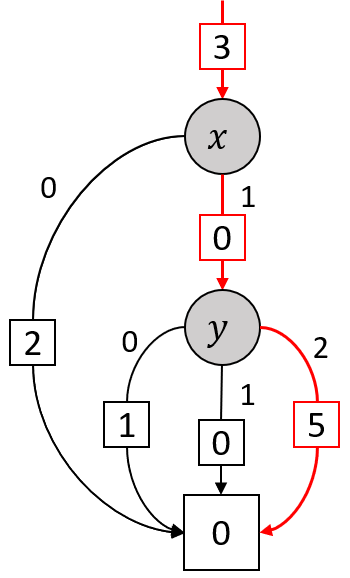
\includegraphics[scale=0.5]{13_3.png}
\end{figure}
\\
%%%%%%%%%%%%%%%%%%%%%  Ejercicio 4 %%%%%%%%%%%%%%%%%%%%%%%%%
\section*{Exercise 13.4 - EVMDD-based action compilation}
Consider again the EVMDD from Exercise 13.3. Assume it encodes the cost $c_{o_1}$ of operator $o_1 = \langle z = 1 \land u = 1, x := 0\rangle$.

\begin{enumerate}[label=\alph*)]
	\item Give the EVMDD-based action compilation of $o_1$ using this EVMDD.
	\begin{align*}
		&O_1^{z=1 \land u=1} = \langle z = 1 \land u = 1 \land \sigma = 0 \land \alpha_{o_1} = 0, \sigma := 1 \land \alpha_{o_1} := 1\rangle & cost=3&\\
		&O_1^{1, x=0} = \langle \alpha_{o_1} = 1 \land x = 0, \alpha_{o_1} := 3 \rangle & cost = 2&\\
		&O_1^{1, x=1} = \langle \alpha_{o_1} = 1 \land x = 1, \alpha_{o_1} := 2 \rangle & cost = 0&\\
		&O_1^{2, y=0} = \langle \alpha_{o_1} = 2 \land y = 0, \alpha_{o_1} := 3 \rangle & cost = 1&\\
		&O_1^{2, y=1} = \langle \alpha_{o_1} = 2 \land y = 1, \alpha_{o_1} := 3 \rangle & cost = 0&\\
		&O_1^{2, y=2} = \langle \alpha_{o_1} = 2 \land y = 2, \alpha_{o_1} := 3 \rangle & cost = 5&\\
		&O_1^{x:=0} = \langle \alpha_{o_1} = 3, x := 0 \land \sigma := 0 \land \alpha_{o_1} := 0 \rangle & cost = 0&\\
	\end{align*}
	\item Let $\Pi = \langle V, I, O, \gamma, (c_o)_{o \in O} \rangle$ with $V = \{x, y, z, u\}$, $\pazocal{D}_x =\pazocal{D}_z = \pazocal{D}_u = \{0, 1\}$ and $\pazocal{D}_y = \{0, 1, 2\}$, initial state $I$ with $I(x) = I(y) = I(z) = I(u) = 1$, operators $O = \{o_1, o_2\}$ with $o_1$ as above and $o_2 = \langle x = 0, z := 0\rangle$ with cost function $c_{o_2} = 1$ and goal formula $\gamma = (z = 0)$. Give an optimal plan $\pi$ for $\Pi$ and an optimal plan $\pi$ for the EVMDD-based action compilation of $\Pi$ and their respective costs.\\
	Optimal plan $\pi$ for $\Pi$\\
	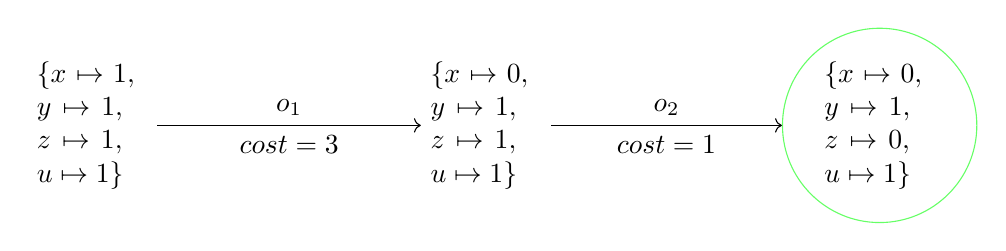
\begin{tikzpicture}[
	node distance = 5cm,
	goalnode/.style={circle, draw=green!60, text width = 4em, minimum size=7mm},
	statenode/.style={rectangle, minimum size=2mm, text width = 4em},
	]
	%Nodes
	\node[statenode]     (i)                      {$\{x \mapsto 1,$ $y \mapsto 1,$ $z \mapsto 1,$ $u \mapsto 1 \} $};
	\node[statenode]     (s1)       [right of = i]  {$\{x \mapsto 0,$ $y \mapsto 1,$ $z \mapsto 1,$ $u \mapsto 1 \} $};
	\node[goalnode]      (s2)       [right of = s1] {$\{x \mapsto 0,$ $y \mapsto 1,$ $z \mapsto 0,$ $u \mapsto 1 \} $};
	
	%Lines
	\draw[->] (i) -- node[below]{$cost = 3$} node[above]{$o_1$} (s1);
	\draw[->] (s1) -- node[below]{$cost = 1$} node[above]{$o_2$} (s2);
	\end{tikzpicture}
	\pagebreak\\
	Optimal plan $\pi$ for $\Pi' = EAC(\Pi)$\\
	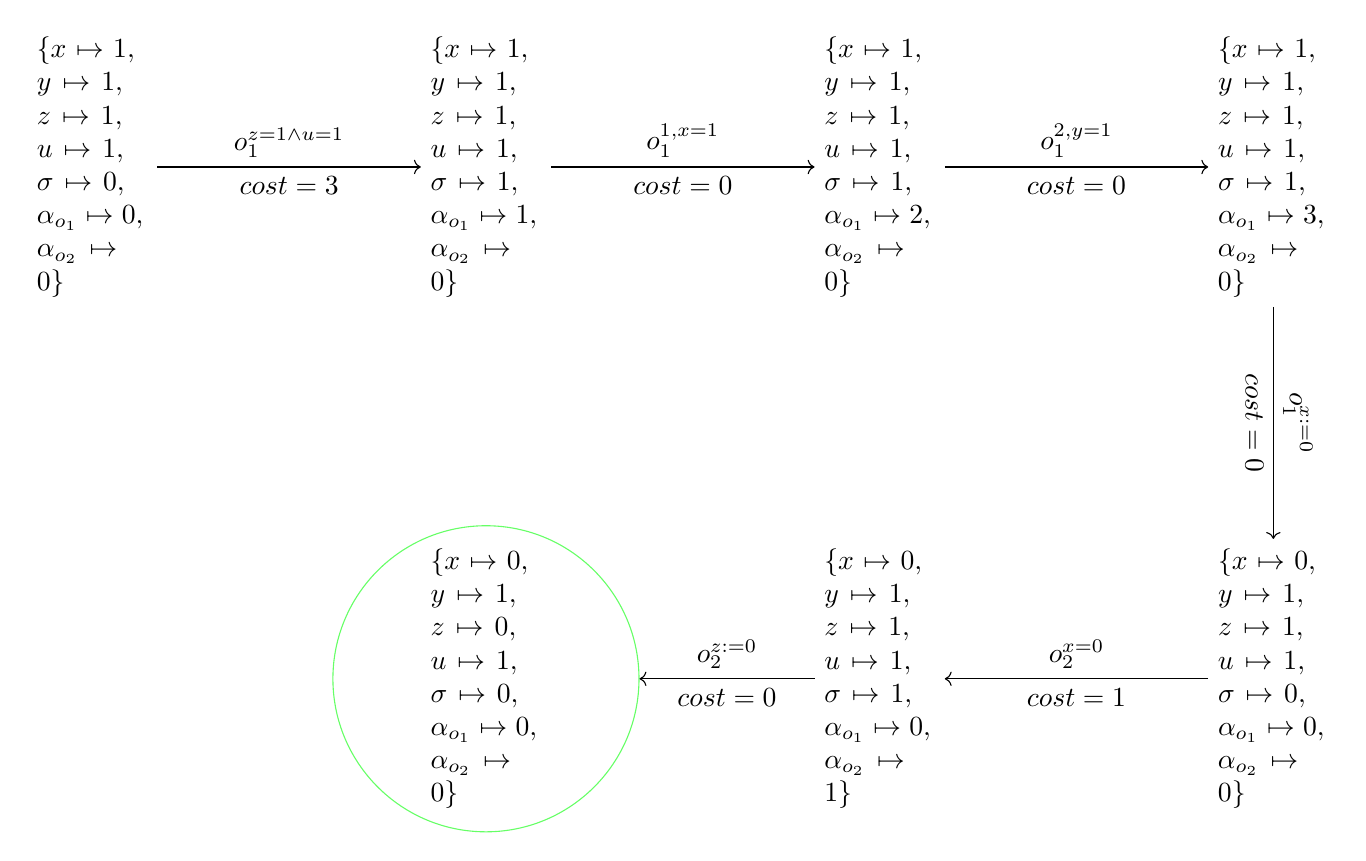
\begin{tikzpicture}[
	node distance = 5cm,
	goalnode/.style={circle, draw=green!60, text width = 4em, minimum size=7mm},
	statenode/.style={rectangle, minimum size=2mm, text width = 4em},
	]
	%Nodes
	\node[statenode]     (i)                      {$\{x \mapsto 1,$ $y \mapsto 1,$ $z \mapsto 1,$ $u \mapsto 1,$ $\sigma \mapsto 0,$ $\alpha_{o_1} \mapsto 0,$ $ \alpha_{o_2} \mapsto 0 \} $};
	\node[statenode]     (s1)       [right of = i] {$\{x \mapsto 1,$ $y \mapsto 1,$ $z \mapsto 1,$ $u \mapsto 1,$ $\sigma \mapsto 1,$ $\alpha_{o_1} \mapsto 1,$ $ \alpha_{o_2} \mapsto 0 \} $};
	\node[statenode]     (s2)       [right of = s1] {$\{x \mapsto 1,$ $y \mapsto 1,$ $z \mapsto 1,$ $u \mapsto 1,$ $\sigma \mapsto 1,$ $\alpha_{o_1} \mapsto 2,$ $ \alpha_{o_2} \mapsto 0 \} $};
	\node[statenode]     (s3)       [right of = s2] {$\{x \mapsto 1,$ $y \mapsto 1,$ $z \mapsto 1,$ $u \mapsto 1,$ $\sigma \mapsto 1,$ $\alpha_{o_1} \mapsto 3,$ $ \alpha_{o_2} \mapsto 0 \} $};
	\node[statenode, yshift = -15mm]     (s4)       [below of = s3] {$\{x \mapsto 0,$ $y \mapsto 1,$ $z \mapsto 1,$ $u \mapsto 1,$ $\sigma \mapsto 0,$ $\alpha_{o_1} \mapsto 0,$ $ \alpha_{o_2} \mapsto 0 \} $};
	\node[statenode]     (s5)       [left of = s4] {$\{x \mapsto 0,$ $y \mapsto 1,$ $z \mapsto 1,$ $u \mapsto 1,$ $\sigma \mapsto 1,$ $\alpha_{o_1} \mapsto 0,$ $ \alpha_{o_2} \mapsto 1 \} $};
	\node[goalnode]      (s6)       [left of = s5] {$\{x \mapsto 0,$ $y \mapsto 1,$ $z \mapsto 0,$ $u \mapsto 1,$ $\sigma \mapsto 0,$ $\alpha_{o_1} \mapsto 0,$ $ \alpha_{o_2} \mapsto 0 \} $};
	
	%Lines
	\draw[->] (i) -- node[below]{$cost = 3$} node[above]{$o_1^{z=1 \land u=1}$} (s1);
	\draw[->] (s1) -- node[below]{$cost = 0$} node[above]{$o_1^{1, x=1}$} (s2);
	\draw[->] (s2) -- node[below]{$cost = 0$} node[above]{$o_1^{2, y=1}$} (s3);
	\draw[->](s3) --node[sloped, below]{$cost = 0$} node[sloped, above]{$o_1^{x\text{:}=0}$} (s4);
	\draw[->] (s4) -- node[below]{$cost = 1$} node[above]{$o_2^{x=0}$} (s5);
	\draw[->] (s5) -- node[below]{$cost = 0$} node[above]{$o_2^{z\text{:}=0}$} (s6);
	\end{tikzpicture}\\	
	We can notice the cost of both plans is the same, 3.
\end{enumerate}
\end{document}